\hypertarget{front-matter}{%
\subsection{Front matter}\label{front-matter}}

title: ``Лабораторная работа №1'' subtitle: ``Отчёт'' author: ``Коровкин
Никита Михайлович''

\hypertarget{generic-otions}{%
\subsection{Generic otions}\label{generic-otions}}

lang: ru-RU toc-title: ``Содержание''

\hypertarget{bibliography}{%
\subsection{Bibliography}\label{bibliography}}

bibliography: bib/cite.bib csl: pandoc/csl/gost-r-7-0-5-2008-numeric.csl

\hypertarget{pdf-output-format}{%
\subsection{Pdf output format}\label{pdf-output-format}}

toc: true \# Table of contents toc-depth: 2 lof: true \# List of figures
lot: true \# List of tables fontsize: 12pt linestretch: 1.5 papersize:
a4 documentclass: scrreprt \#\# I18n polyglossia polyglossia-lang: name:
russian options: - spelling=modern - babelshorthands=true
polyglossia-otherlangs: name: english \#\# I18n babel babel-lang:
russian babel-otherlangs: english \#\# Fonts mainfont: IBM Plex Serif
romanfont: IBM Plex Serif sansfont: IBM Plex Sans monofont: IBM Plex
Mono mathfont: STIX Two Math mainfontoptions:
Ligatures=Common,Ligatures=TeX,Scale=0.94 romanfontoptions:
Ligatures=Common,Ligatures=TeX,Scale=0.94 sansfontoptions:
Ligatures=Common,Ligatures=TeX,Scale=MatchLowercase,Scale=0.94
monofontoptions: Scale=MatchLowercase,Scale=0.94,FakeStretch=0.9
mathfontoptions: \#\# Biblatex biblatex: true biblio-style:
``gost-numeric'' biblatexoptions: - parentracker=true - backend=biber -
hyperref=auto - language=auto - autolang=other* - citestyle=gost-numeric
\#\# Pandoc-crossref LaTeX customization figureTitle: ``Рис.''
tableTitle: ``Таблица'' listingTitle: ``Листинг'' lofTitle: ``Список
иллюстраций'' lotTitle: ``Список таблиц'' lolTitle: ``Листинги'' \#\#
Misc options indent: true header-includes: -

\usepackage{indentfirst}

\begin{itemize}
\item
  \usepackage{float}

  \hypertarget{keep-figures-where-there-are-in-the-text}{%
  \section{keep figures where there are in the
  text}\label{keep-figures-where-there-are-in-the-text}}

  \begin{itemize}
  \item ~
    \hypertarget{keep-figures-where-there-are-in-the-text-1}{%
    \subsection{\texorpdfstring{\floatplacement{figure}{h!} \# keep
    figures where there are in the
    text}{ \# keep figures where there are in the text}}\label{keep-figures-where-there-are-in-the-text-1}}
  \end{itemize}
\end{itemize}

\hypertarget{ux446ux435ux43bux44c-ux440ux430ux431ux43eux442ux44b}{%
\section{Цель
работы}\label{ux446ux435ux43bux44c-ux440ux430ux431ux43eux442ux44b}}

Целью данной работы является приобретение практических навыков установки
операционной системы на виртуальную машину, настройки минимально
необходимых для дальнейшей работы сервисов.

\hypertarget{ux437ux430ux434ux430ux43dux438ux435}{%
\section{Задание}\label{ux437ux430ux434ux430ux43dux438ux435}}

Установка операционной системы Установка драйверов для VirtualBox
Настройка раскладки клавиатуры Установка имени пользователя и названия
хоста Подключение общей папки Установка программного обеспечения для
создания документации Домашнее задание

\hypertarget{ux432ux44bux43fux43eux43bux43dux435ux43dux438ux435-ux43bux430ux431ux43eux440ux430ux442ux43eux440ux43dux43eux439-ux440ux430ux431ux43eux442ux44b}{%
\section{Выполнение лабораторной
работы}\label{ux432ux44bux43fux43eux43bux43dux435ux43dux438ux435-ux43bux430ux431ux43eux440ux430ux442ux43eux440ux43dux43eux439-ux440ux430ux431ux43eux442ux44b}}

В первую очередь нам необходимо создать виртуальную машину. Она уже была
создана во время предыдущего семестра с помощью utm.(рис.
{[}-@fig:001{]}).

\begin{figure}
\hypertarget{fig:001}{%
\centering

\includegraphics[width=0.7\textwidth,height=\textheight]{image/1.png}
\caption{Установка виртуальной машины}\label{fig:001}
}
\end{figure}

Теперь войдем в наш имеющийся заранее аккаунт.(рис. {[}-@fig:002{]}).

\begin{figure}
\hypertarget{fig:002}{%
\centering
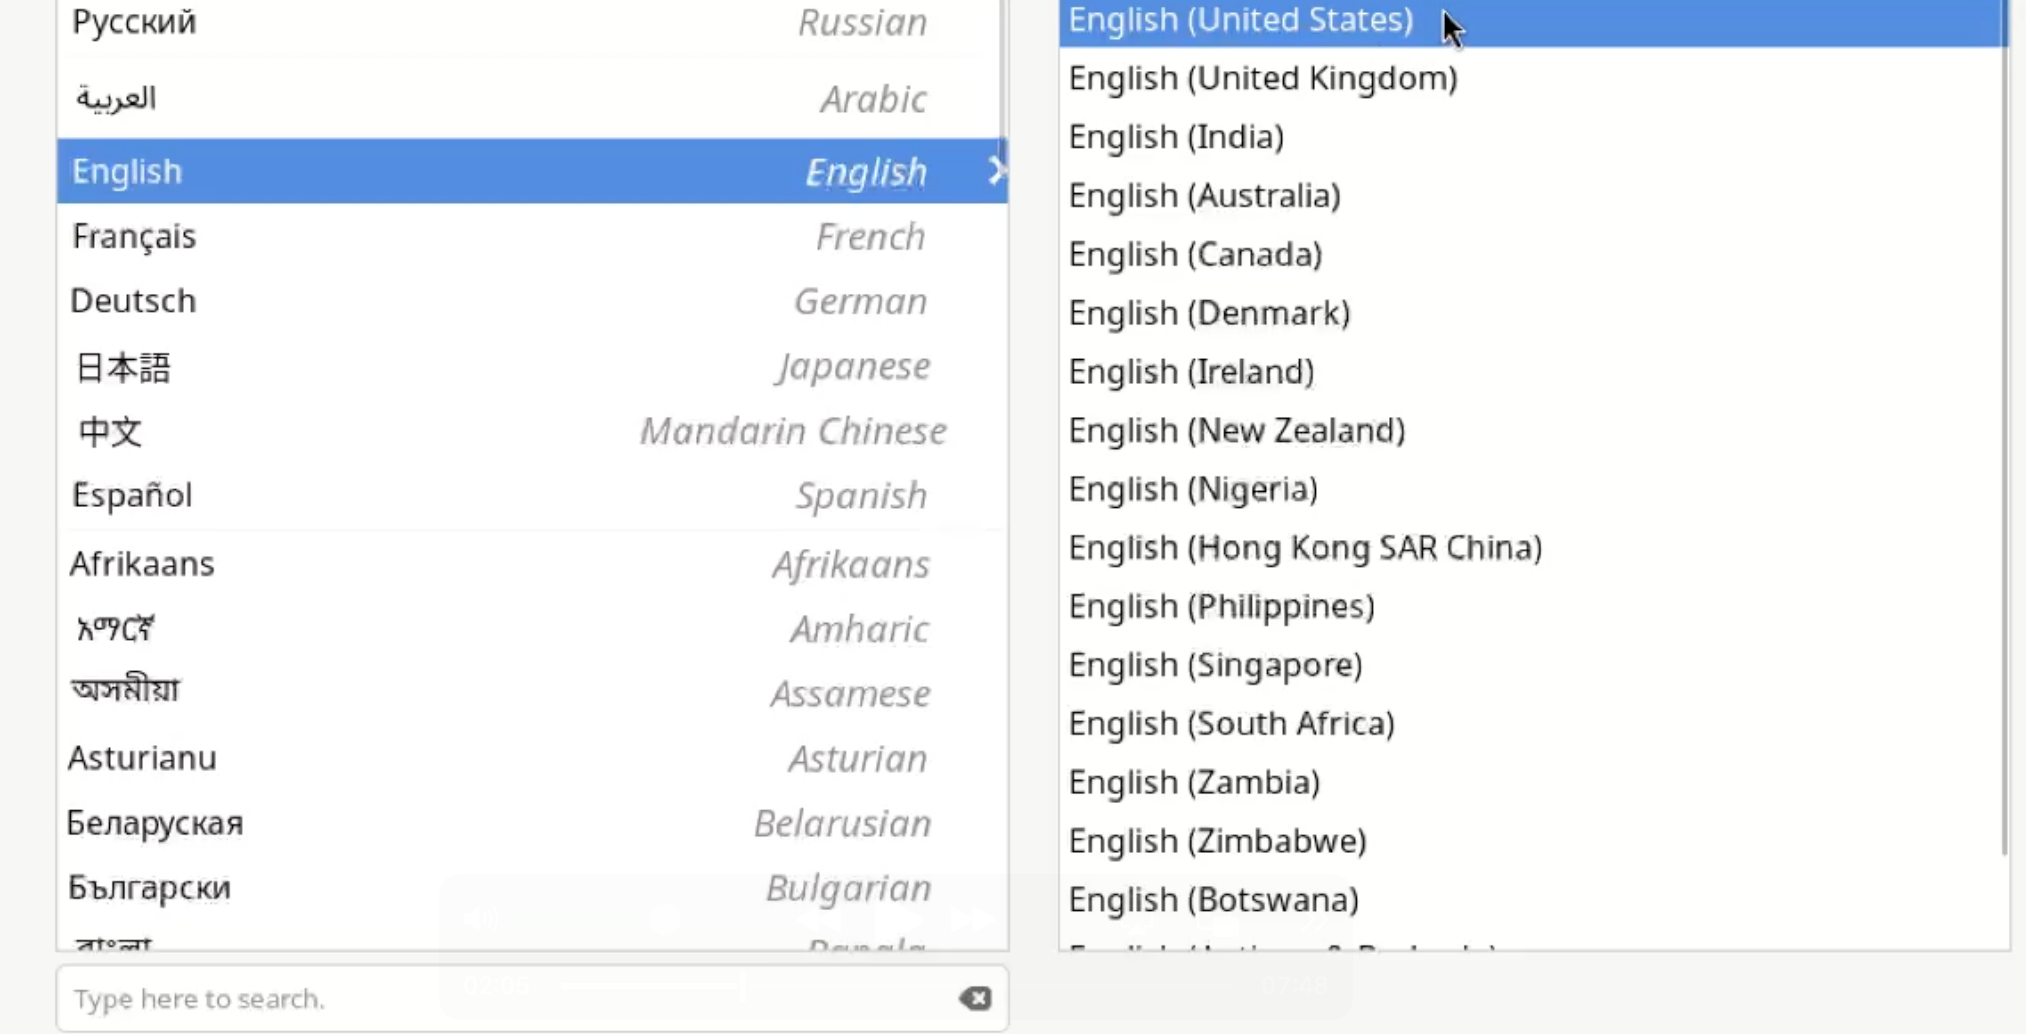
\includegraphics[width=0.7\textwidth,height=\textheight]{image/2.jpeg}
\caption{Вход в аккаунт}\label{fig:002}
}
\end{figure}

Теперь установим менеджер окон sway {[}-@fig:003{]}

\begin{figure}
\hypertarget{fig:003}{%
\centering
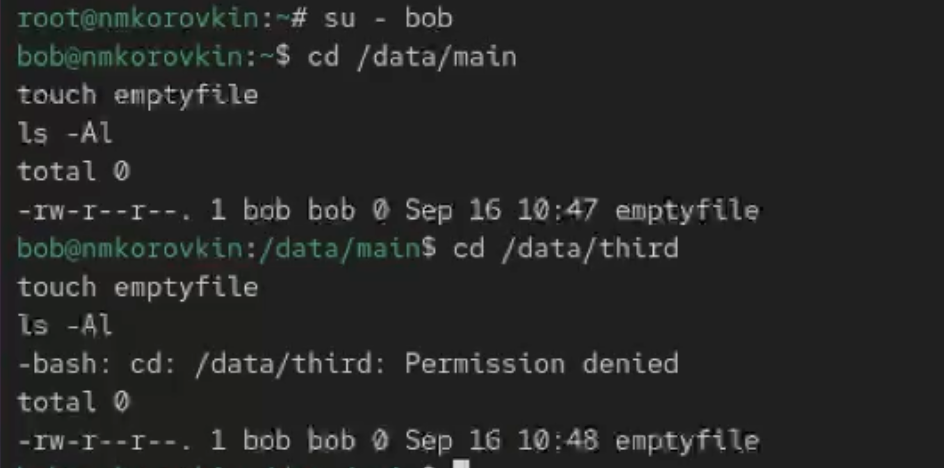
\includegraphics[width=0.7\textwidth,height=\textheight]{image/3.jpeg}
\caption{Менеджер окон}\label{fig:003}
}
\end{figure}

После этого нам необходимо получить особые права пользователя.(рис.
{[}-@fig:004{]}).

\begin{figure}
\hypertarget{fig:004}{%
\centering
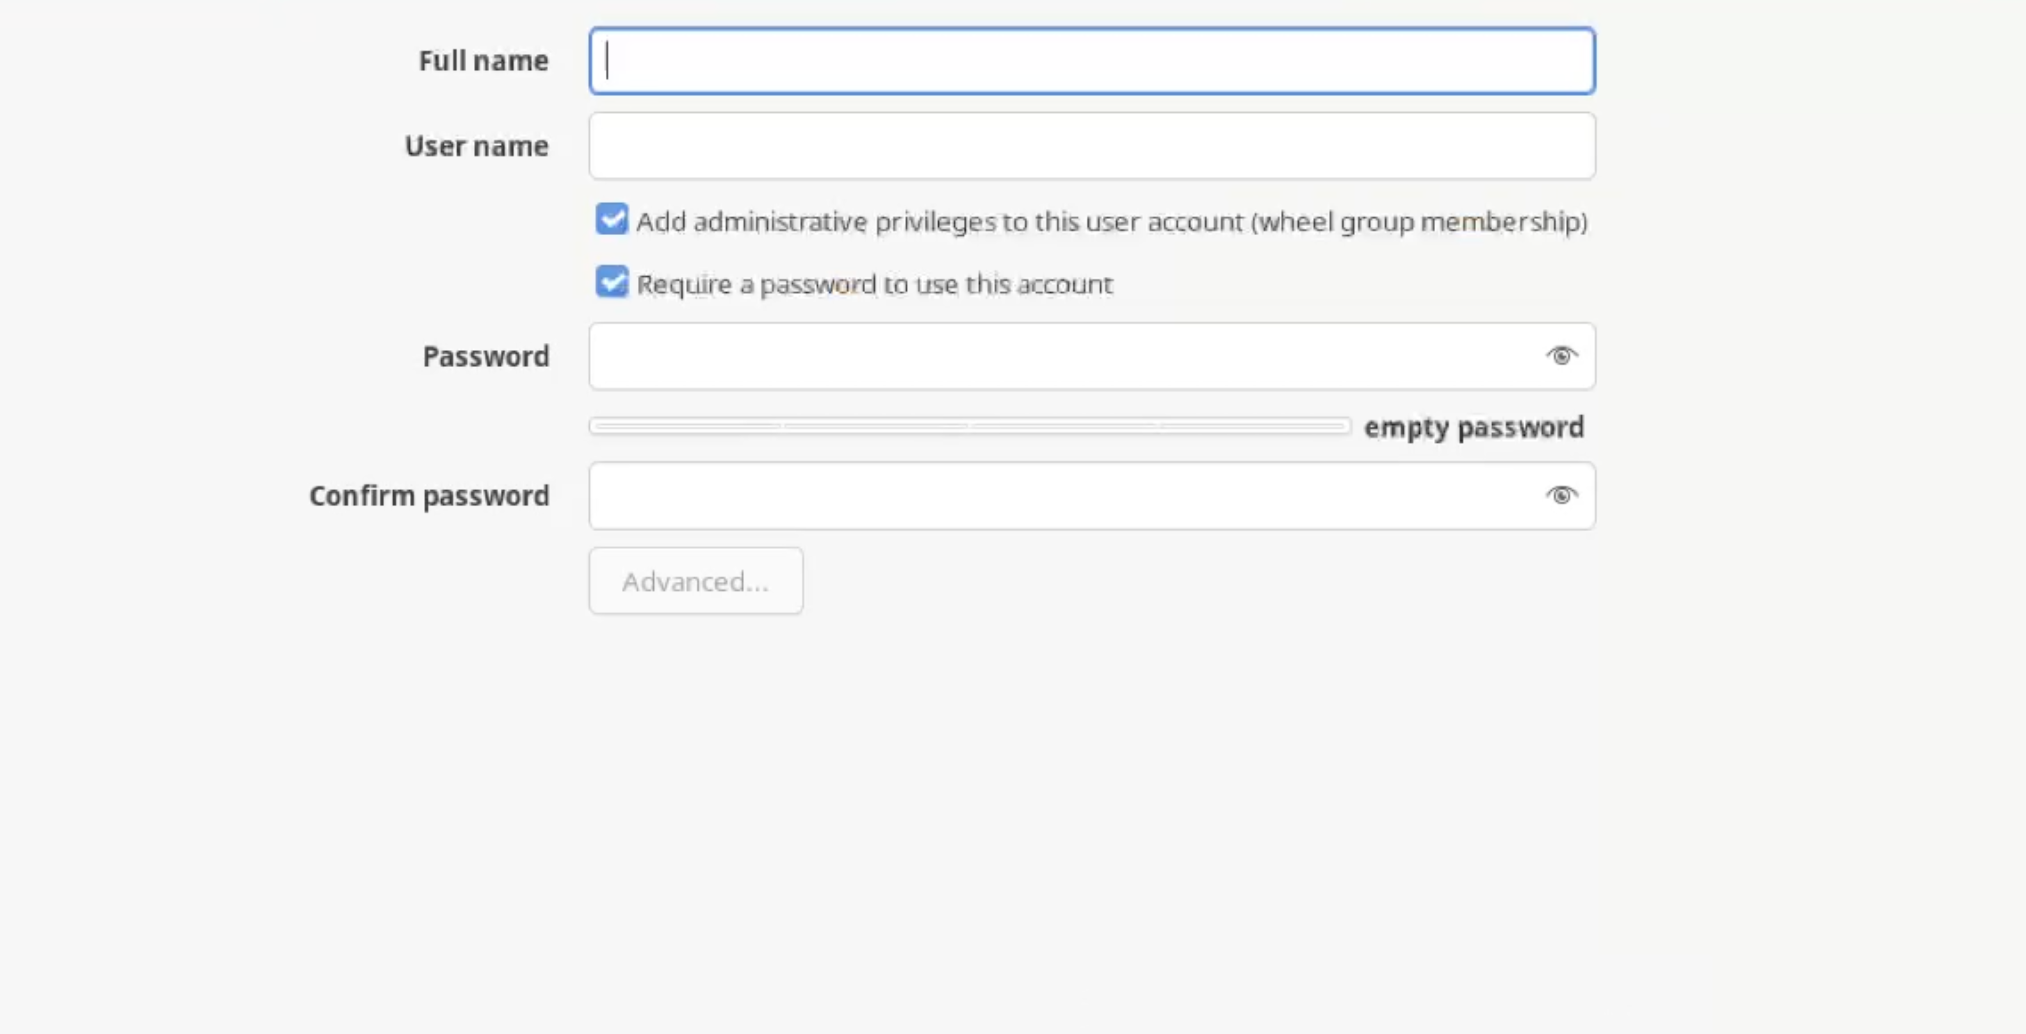
\includegraphics[width=0.7\textwidth,height=\textheight]{image/5.png}
\caption{особые права пользователя}\label{fig:004}
}
\end{figure}

Обновим все пакеты с помощью dnf.(рис. {[}-@fig:005{]}).

\begin{figure}
\hypertarget{fig:005}{%
\centering
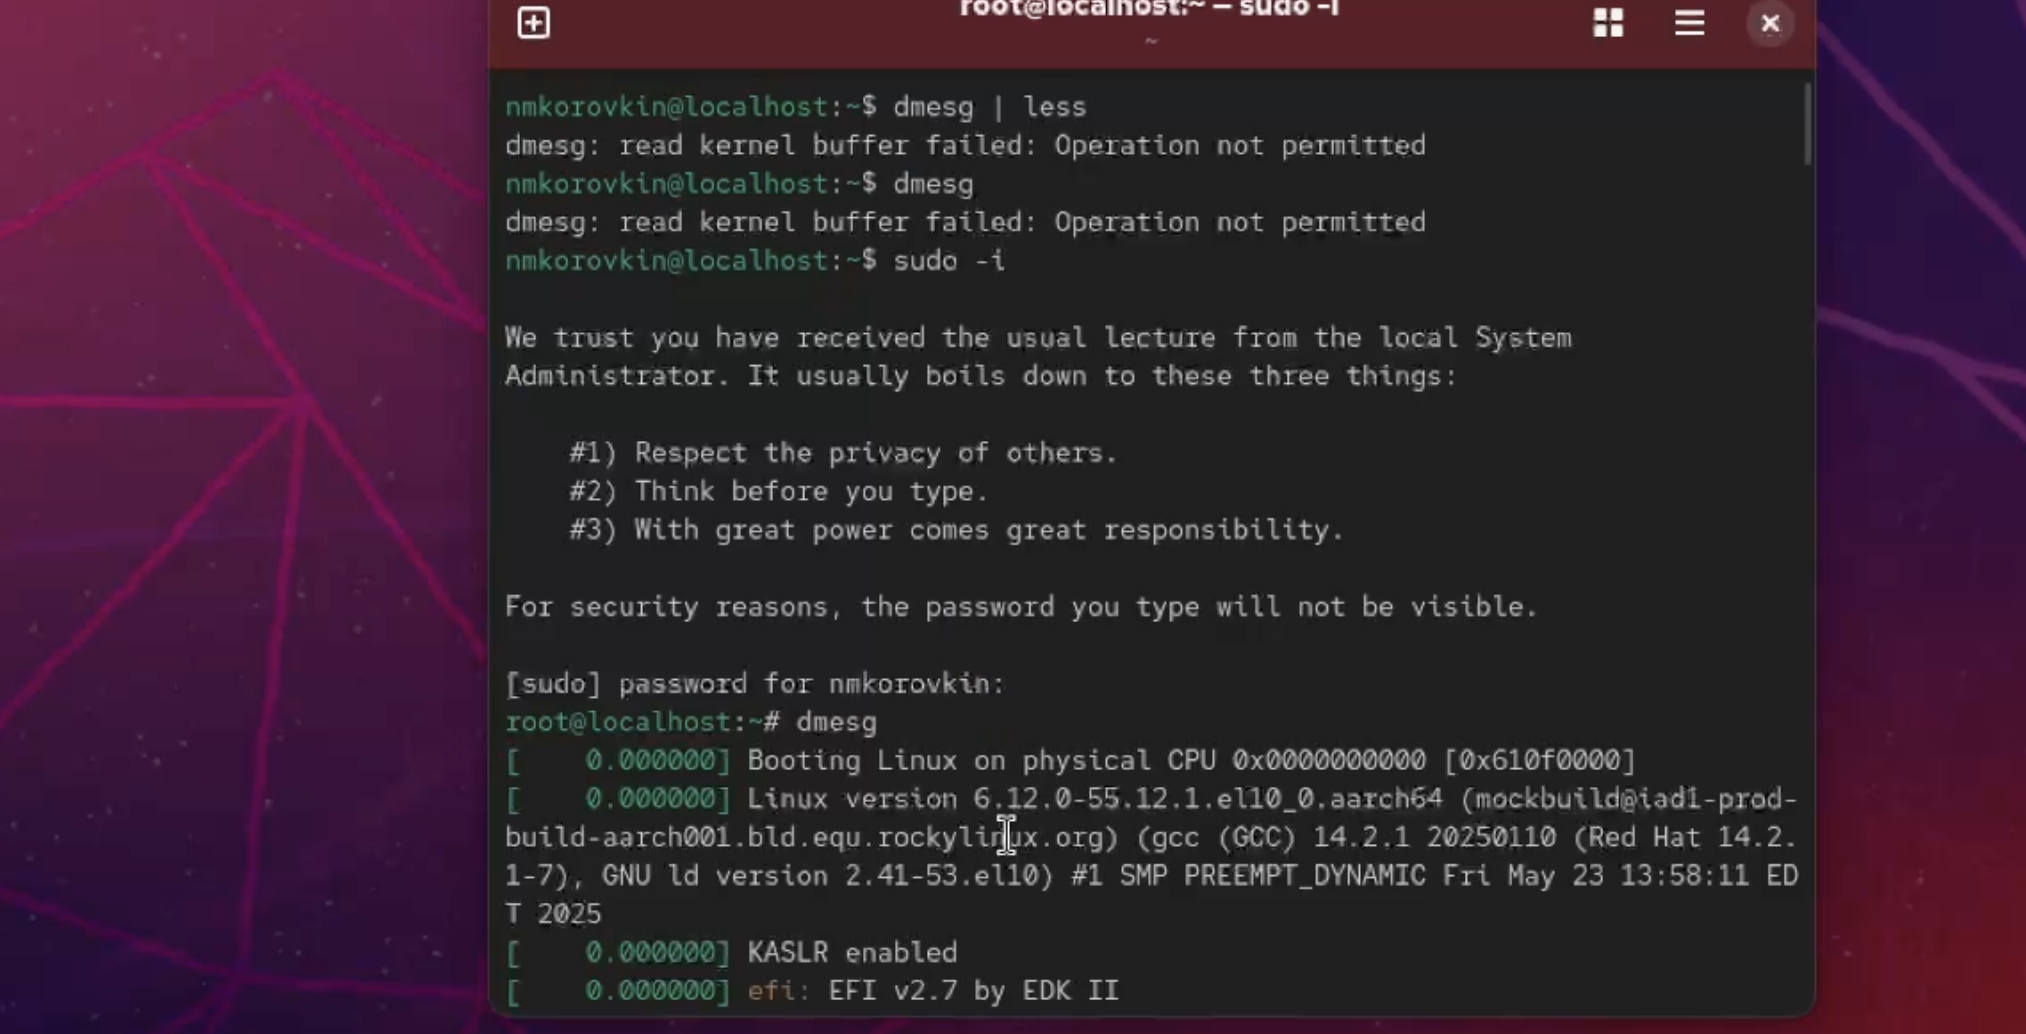
\includegraphics[width=0.7\textwidth,height=\textheight]{image/7.jpg}
\caption{Обновление пакетов}\label{fig:005}
}
\end{figure}

Установим tmux с помощью dnf. Все остальные программы также в основном
устанавливаются через dnf.(рис. {[}-@fig:006{]}).

\begin{figure}
\hypertarget{fig:006}{%
\centering
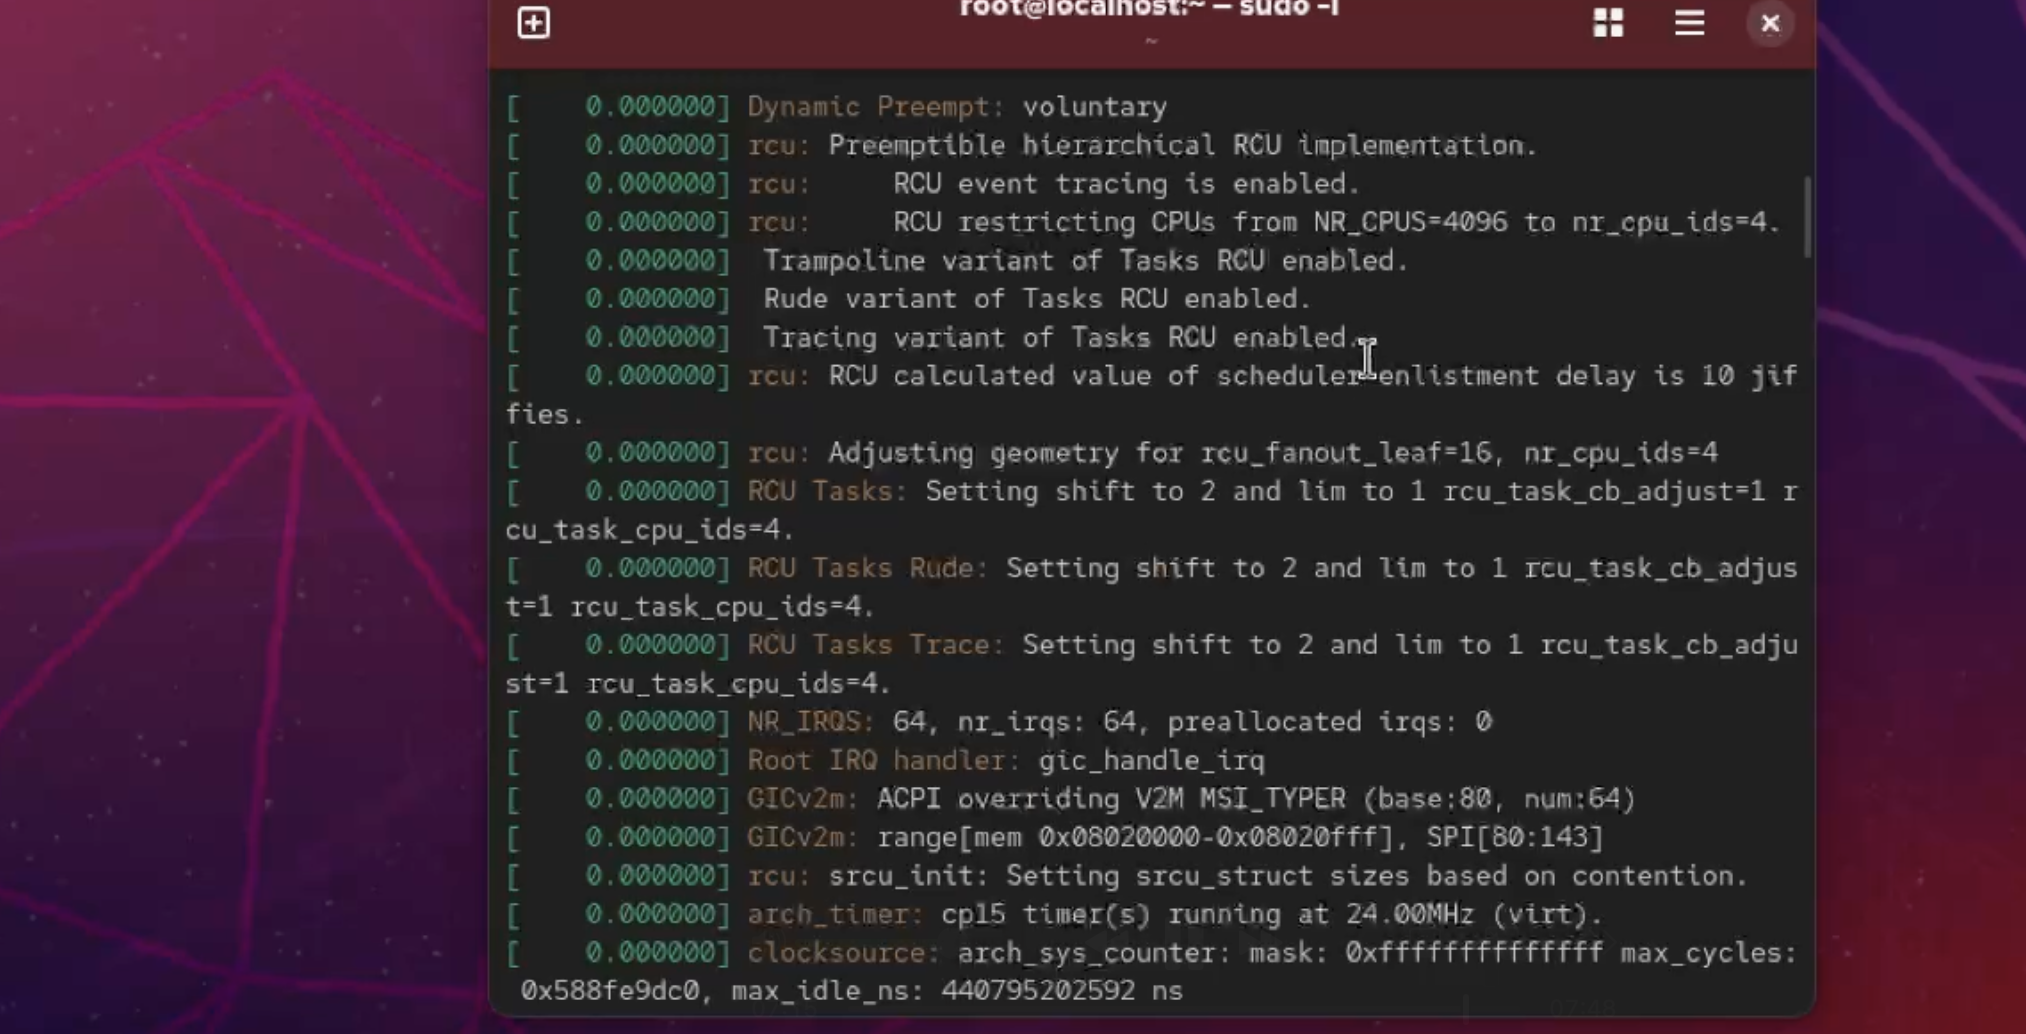
\includegraphics[width=0.7\textwidth,height=\textheight]{image/8.jpg}
\caption{Установим tmux}\label{fig:006}
}
\end{figure}

Установим dnf-automatic (рис. {[}-@fig:007{]}).

\begin{figure}
\hypertarget{fig:007}{%
\centering
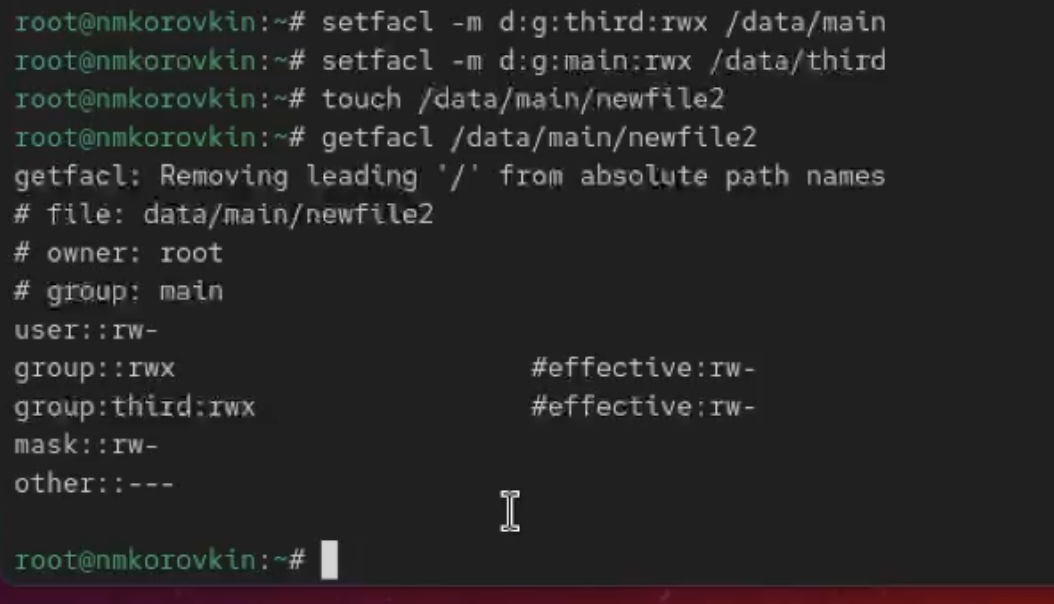
\includegraphics[width=0.7\textwidth,height=\textheight]{image/10.jpg}
\caption{Установим dnf-automatic}\label{fig:007}
}
\end{figure}

Теперь нам нужно будет работать с файлом конфигурации клавиатуры.(рис.
{[}-@fig:008{]}).

\begin{figure}
\hypertarget{fig:008}{%
\centering
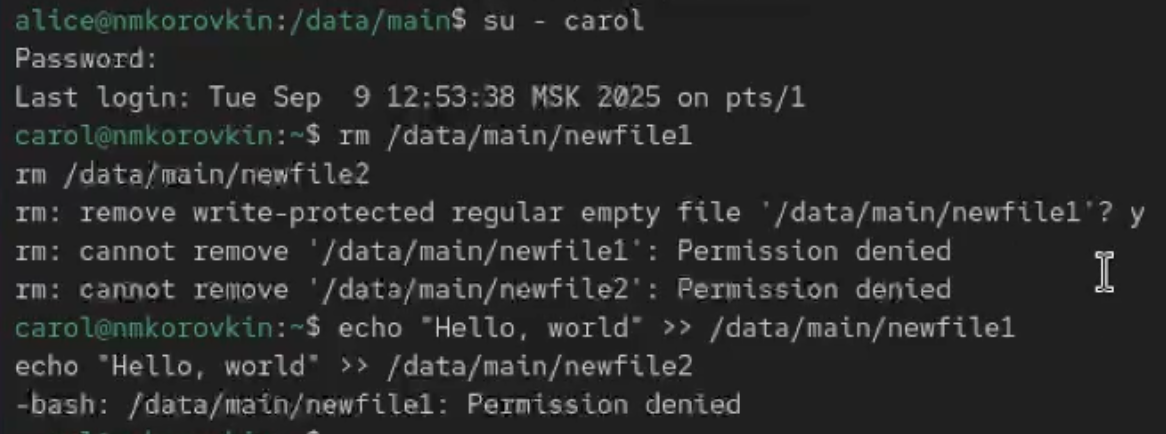
\includegraphics[width=0.7\textwidth,height=\textheight]{image/11.jpg}
\caption{Создаем файл конфигурации}\label{fig:008}
}
\end{figure}

Вставим следующую строчку в созданный нами файл.(рис. {[}-@fig:009{]}).

\begin{figure}
\hypertarget{fig:009}{%
\centering
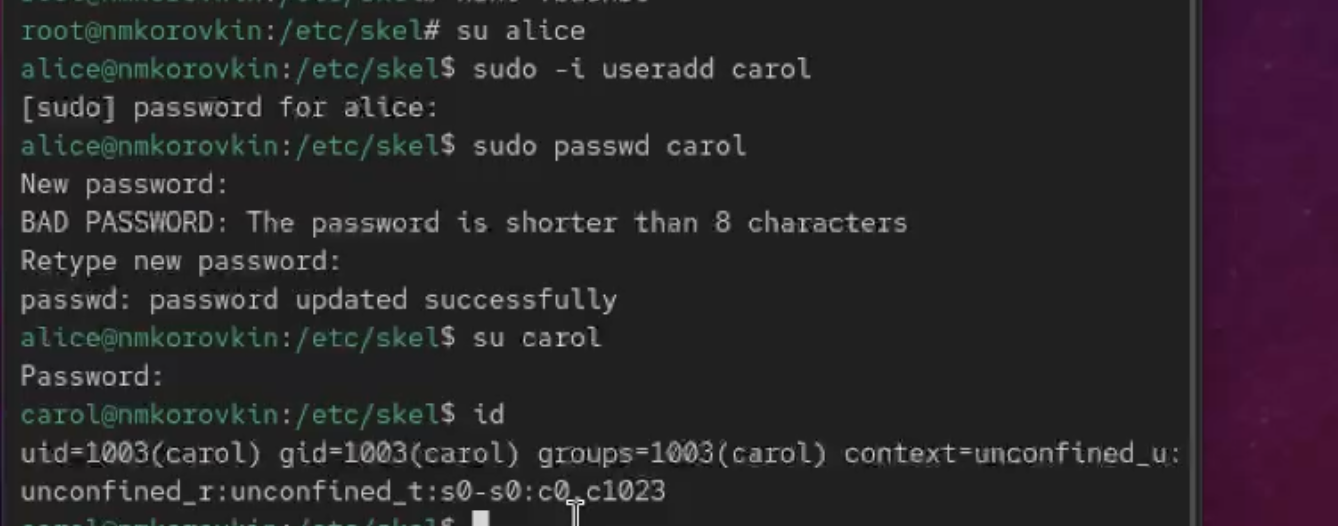
\includegraphics[width=0.7\textwidth,height=\textheight]{image/12.jpg}
\caption{Редактируем файл}\label{fig:009}
}
\end{figure}

Редактируем еще один файл.(рис. {[}-@fig:010{]}).

\begin{figure}
\hypertarget{fig:010}{%
\centering
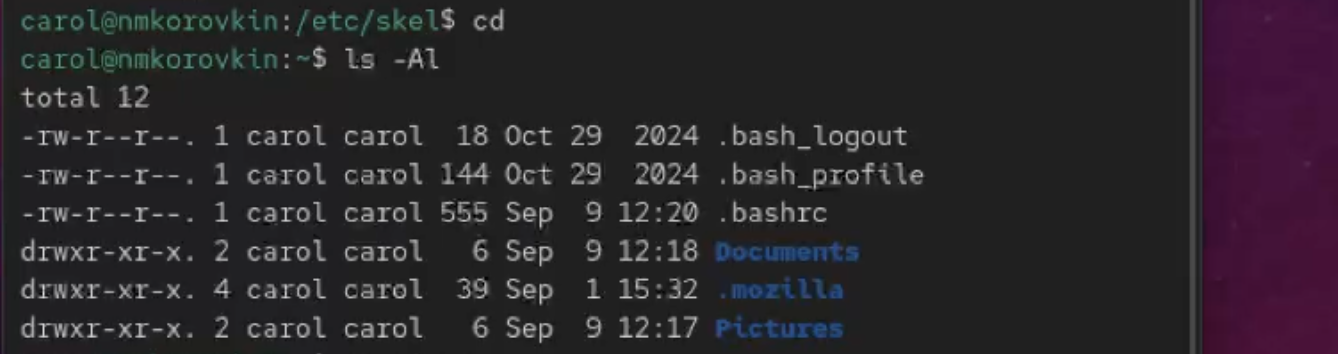
\includegraphics[width=0.7\textwidth,height=\textheight]{image/13.jpg}
\caption{Редактируем следующий файл}\label{fig:010}
}
\end{figure}

Перезагружаем систему.(рис. {[}-@fig:011{]}).

\begin{figure}
\hypertarget{fig:011}{%
\centering
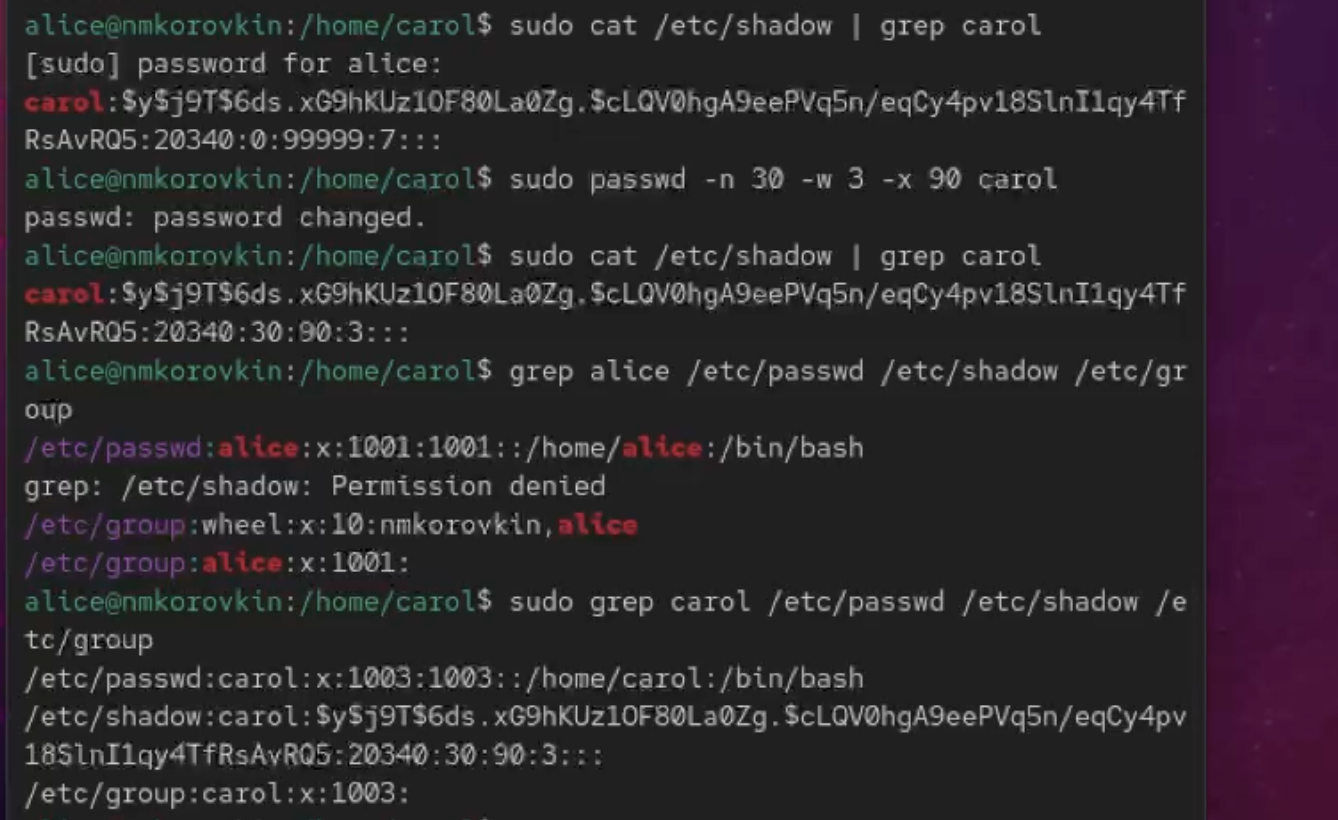
\includegraphics[width=0.7\textwidth,height=\textheight]{image/14.jpg}
\caption{Перезагружаем систему}\label{fig:011}
}
\end{figure}

Теперь добавим пользователя.(рис. {[}-@fig:012{]}).

\begin{figure}
\hypertarget{fig:012}{%
\centering
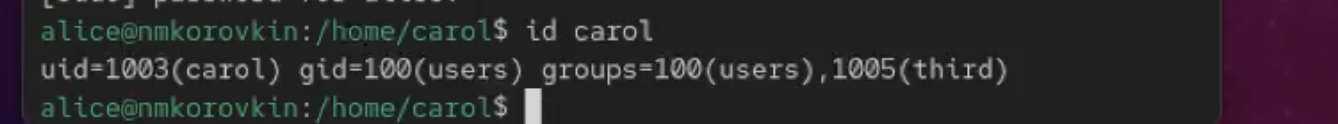
\includegraphics[width=0.7\textwidth,height=\textheight]{image/16.jpg}
\caption{Добавляем пользователя}\label{fig:012}
}
\end{figure}

Заполним имя и пароль.(рис. {[}-@fig:013{]}).

\begin{figure}
\hypertarget{fig:013}{%
\centering
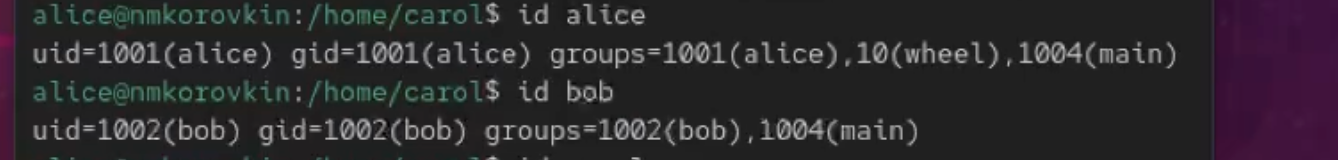
\includegraphics[width=0.7\textwidth,height=\textheight]{image/17.jpg}
\caption{Заполнение имени и пароля}\label{fig:013}
}
\end{figure}

Установим хост.(рис. {[}-@fig:014{]}).

\begin{figure}
\hypertarget{fig:014}{%
\centering
\includegraphics[width=0.7\textwidth,height=\textheight]{image/18.jpg}
\caption{Установка хоста}\label{fig:014}
}
\end{figure}

Проверим, получилось ли.(рис. {[}-@fig:015{]}).

\begin{figure}
\hypertarget{fig:015}{%
\centering
\includegraphics[width=0.7\textwidth,height=\textheight]{image/21.jpg}
\caption{Проверка}\label{fig:015}
}
\end{figure}

Далее нам нужно установить Pandoc и Texlive.Так как они уже были
установлены в предыдущем семестре, проверим точно ли они у нас есть(рис.
{[}-@fig:016{]} ).

\begin{figure}
\hypertarget{fig:016}{%
\centering
\includegraphics[width=0.7\textwidth,height=\textheight]{image/23.jpg}
\caption{Проверка Pandoc и Texlive}\label{fig:016}
}
\end{figure}

Все верно.

\#Домашнее задание

Теперь предстоит проверить версию ядра, гипервизор, модель процессора,
его частоту и количество оперативной памяти.(рис.
{[}-@fig:017{]},{[}-@fig:018{]},{[}-@fig:019{]})

\begin{figure}
\hypertarget{fig:017}{%
\centering
\includegraphics[width=0.7\textwidth,height=\textheight]{image/24.jpg}
\caption{Находим информацию о компьютере}\label{fig:017}
}
\end{figure}

\begin{figure}
\hypertarget{fig:018}{%
\centering
\includegraphics[width=0.7\textwidth,height=\textheight]{image/25.jpg}
\caption{Находим информацию о компьютере}\label{fig:018}
}
\end{figure}

\begin{figure}
\hypertarget{fig:019}{%
\centering
\includegraphics[width=0.7\textwidth,height=\textheight]{image/26.jpg}
\caption{Находим информацию о компьютере}\label{fig:019}
}
\end{figure}

Некоторые команды не сработали из-за особенностей чипа m2.

Работа выполнена верно.

\#Выводы

В ходе выполнения работы Были получены навыки работы и знания о системе
Fedora Sway, была проведена установка системы, установлены все
необходимые для последующей работы пакеты и произведена базовая
настройка системы.

\#Ответы на контрольные вопросы

\begin{enumerate}
\def\labelenumi{\arabic{enumi})}
\tightlist
\item
  Какую информацию содержит учётная запись пользователя?
\end{enumerate}

\begin{itemize}
\tightlist
\item
  Логин пользователя, пароль пользователя, его ID, ID его группы,
  дополнительная информация (настоящее имя, почта), домашний каталог
  пользователя
\end{itemize}

\begin{enumerate}
\def\labelenumi{\arabic{enumi})}
\setcounter{enumi}{1}
\tightlist
\item
  Укажите команды терминала и приведите примеры:
\end{enumerate}

\begin{itemize}
\item
  Для перемещения по файловой системе Используется команда cd. Например:
  cd \textasciitilde{} - переместиться в домашний каталог
\item
  Для просмотра содержимого каталога Используется команда ls. Например:
  ls / - посмотреть содержимое корневого каталога
\item
  Для определения объёма каталога Используется команда du. Например: du
  -- выводит размер всех подкаталогов и файлов в каталоге
\item
  Для создания / удаления каталогов / файлов -Для создания файлов:
  touch. Например: touch /test.txt -- создать файл test.txt в корне -Для
  удаления файлов: rm. Например: rm /test.txt -- удалить файл test.txt в
  корне -Для создания каталогов: mkdir. Например: mkdir /test -- создать
  папку test в корне -Для удаления каталогов: rmdir. Например: rmdir
  /test -- удалить папку test в корне
\end{itemize}

\begin{enumerate}
\def\labelenumi{\arabic{enumi})}
\setcounter{enumi}{2}
\tightlist
\item
  Что такое файловая система? Приведите примеры с краткой
  характеристикой.
\end{enumerate}

\begin{itemize}
\tightlist
\item
  Файловая система -- это система организации файлов в операционной
  системе. Например: FAT -- Система, созданная Microsoft, не
  поддерживала шифрование, права пользователей к файлам и не имела
  возможности журналирования EXT4 -- Более современная файловая система,
  которая нынче активно используется в linux, поддерживает
  журналирование, шифрование и права пользователей к файлам
\end{itemize}

\begin{enumerate}
\def\labelenumi{\arabic{enumi})}
\setcounter{enumi}{3}
\tightlist
\item
  Как посмотреть, какие файловые системы подмонтированы в ОС?
\end{enumerate}

\begin{itemize}
\tightlist
\item
  Можно посмотреть с помощью утилиты df
\end{itemize}

\begin{enumerate}
\def\labelenumi{\arabic{enumi})}
\setcounter{enumi}{4}
\tightlist
\item
  Как удалить зависший процесс?
\end{enumerate}

\begin{itemize}
\tightlist
\item
  По PID с помощью команды kill, либо по имени с помощью команды killall
\end{itemize}
